%# -*- coding: utf-8-unix -*-
% !TEX program = xelatex
%%==================================================
%% thesis.tex
%%==================================================

\documentclass[bachelor, openany, oneside]{ssputhesis}

% 逐个导入参考文献数据库
\addbibresource{bib/thesis.bib}

%# -*- coding: utf-8-unix -*-
% !TEX program = xelatex
% !TEX root = ../thesis.tex
% !TEX encoding = UTF-8 Unicode
%TC:ignore
\title{基于Latex的论文模版}
\author{某\quad{}某}
\advisor{某某老师}
% \coadvisor{某某教授}
\defenddate{2019年5月8日}
\coursename{某某课程}
\school{上海第二工业大学}
\institute{某某学部}
\studentnumber{12345678901}
\cnacademicdegree{工学硕士}
\major{某某专业}
\class{某某班级}
\entrancetime{某某级}
\keywords{SSPU;Latex;论文}

\englishtitle{iOS-Based Task Plan and Time Management System}
\englishauthor{\textsc{Mo Mo}}
\englishadvisor{Prof. \textsc{Mou Mou}}
% \englishcoadvisor{Prof. \textsc{Uom Uom}}
\englishschool{Shanghai Jiao Tong University}
\englishinstitute{\textsc{Depart of XXX, School of XXX} \\
  \textsc{Shanghai Jiao Tong University} \\
  \textsc{Shanghai, P.R.China}}
\englishinstitutemaster{Depart of XXX, \\ School of XXX}
\englishmajor{A Very Important Major}
\englishdate{Dec. 17th, 2014}
\enacademicdegree{Master of Engineering}
\englishstudentid{0010900990}
\englishkeywords{SSPU, Latex, Thesis}
%TC:endignore
  % NOTE: the enclosed commands must be executed in preamble

\begin{document}

% 无编号内容:中英文论文封面、授权页
\maketitle

\makeatletter % 使用 @ 字符

\makeDeclareOriginal
\frontmatter % 使用罗马数字对前言编号

% 摘要
%# -*- coding: utf-8-unix -*-
% !TEX program = xelatex
% !TEX root = ../thesis.tex
% !TEX encoding = UTF-8 Unicode
%%==================================================
%% abstract.tex for SJTU Master Thesis
%%==================================================

\begin{abstract}



\end{abstract}

\begin{englishabstract}

An imperial edict issued in 1896 by Emperor Guangxu, established Nanyang Public School in Shanghai. The normal school, school of foreign studies, middle school and a high school were established. Sheng Xuanhuai, the person responsible for proposing the idea to the emperor, became the first president and is regarded as the founder of the university.

During the 1930s, the university gained a reputation of nurturing top engineers. After the foundation of People's Republic, some faculties were transferred to other universities. A significant amount of its faculty were sent in 1956, by the national government, to Xi'an to help build up Xi'an Jiao Tong University in western China. Afterwards, the school was officially renamed Shanghai Jiao Tong University.

Since the reform and opening up policy in China, SJTU has taken the lead in management reform of institutions for higher education, regaining its vigor and vitality with an unprecedented momentum of growth. SJTU includes five beautiful campuses, Xuhui, Minhang, Luwan Qibao, and Fahua, taking up an area of about 3,225,833 m2. A number of disciplines have been advancing towards the top echelon internationally, and a batch of burgeoning branches of learning have taken an important position domestically.

Today SJTU has 31 schools (departments), 63 undergraduate programs, 250 masters-degree programs, 203 Ph.D. programs, 28 post-doctorate programs, and 11 state key laboratories and national engineering research centers.

SJTU boasts a large number of famous scientists and professors, including 35 academics of the Academy of Sciences and Academy of Engineering, 95 accredited professors and chair professors of the "Cheung Kong Scholars Program" and more than 2,000 professors and associate professors.

Its total enrollment of students amounts to 35,929, of which 1,564 are international students. There are 16,802 undergraduates, and 17,563 masters and Ph.D. candidates. After more than a century of operation, Jiao Tong University has inherited the old tradition of "high starting points, solid foundation, strict requirements and extensive practice." Students from SJTU have won top prizes in various competitions, including ACM International Collegiate Programming Contest, International Mathematical Contest in Modeling and Electronics Design Contests. Famous alumni include Jiang Zemin, Lu Dingyi, Ding Guangen, Wang Daohan, Qian Xuesen, Wu Wenjun, Zou Taofen, Mao Yisheng, Cai Er, Huang Yanpei, Shao Lizi, Wang An and many more. More than 200 of the academics of the Chinese Academy of Sciences and Chinese Academy of Engineering are alumni of Jiao Tong University.

\end{englishabstract}



% 目录
\tableofcontents

\makeatother
\mainmatter % 使用阿拉伯数字对正文编号

% 正文内容
%# -*- coding: utf-8-unix -*-
% !TEX program = xelatex
% !TEX root = ../thesis.tex
% !TEX encoding = UTF-8 Unicode
%%==================================================
%% chapter01.tex for SJTU Master Thesis
%%==================================================

%\bibliographystyle{sspu2}%[此处用于每章都生产参考文献]
\chapter{这是什么}
\label{chap:intro}

这是上海交通大学(非官方)学位论文 \LaTeX 模板,当前版本是 \version 。

最早的一版学位模板是一位热心的物理系同学制作的。
那份模板参考了自动化所学位论文模板,使用了CASthesis.cls文档类,中文字符处理则采用当时最为流行的 \CJKLaTeX 方案。
我根据交大研究生院对学位论文的要求
\footnote{\url{http://www.gs.sspu.edu.cn/policy/fileShow.ahtml?id=130}}
,结合少量个人审美喜好,完成了一份基本可用的交大 \LaTeX 学位论文模板。
但是,搭建一个 \CJKLaTeX 环境并不简单,单单在Linux下配置环境和添加中文字体,就足够让新手打退堂鼓。
在William Wang的建议下,我开始着手把模板向 \XeTeX 引擎移植。
他完成了最初的移植,多亏了他出色的工作,后续的改善工作也得以顺利进行。

随着我对 \LaTeX 系统认知增加,我又断断续续做了一些完善模板的工作,在原有硕士学位论文模板的基础上完成了交大学士和博士学位论文模板。

现在,交大学位论文模板SJTUTHesis代码在github
\footnote{\url{https://github.com/sspug/SJTUThesis}}
上维护。
你可以\href{https://github.com/sspug/SJTUThesis/issues}{在github上开issue}
、或者在\href{https://bbs.sspu.edu.cn/bbsdoc?board=TeX_LaTeX}{水源LaTeX版}发帖来反映遇到的问题。

\section{使用模板}

\subsection{准备工作}
\label{sec:requirements}

要使用这个模板撰写学位论文,需要在\emph{TeX系统}、\emph{TeX技能}上有所准备。

\begin{itemize}[noitemsep,topsep=0pt,parsep=0pt,partopsep=0pt]
	\item {\TeX}系统:所使用的{\TeX}系统要支持 \XeTeX 引擎,且带有ctex 2.x宏包,以2017年或更新版本的\emph{完整}TeXLive、MacTeX发行版为佳。
	\item TeX技能:尽管提供了对模板的必要说明,但这不是一份“ \LaTeX 入门文档”。在使用前请先通读其他入门文档。
	\item 针对Windows用户的额外需求:学位论文模本分别使用git和GNUMake进行版本控制和构建,建议从Cygwin\footnote{\url{http://cygwin.com}}安装这两个工具。
\end{itemize}

\subsection{模板选项}
\label{sec:thesisoption}

ssputhesis提供了一些常用选项,在thesis.tex在导入ssputhesis模板类时,可以组合使用。
这些选项包括:

\begin{itemize}[noitemsep,topsep=0pt,parsep=0pt,partopsep=0pt]
	\item 学位类型:bachelor(学位)、master(硕士)、doctor(博士),是必选项。
	\item 中文字体:fandol(Fandol 开源字体)、windows(Windows 系统下的中文字体)、mac(macOS 系统下的华文字体)、ubuntu(Ubuntu 系统下的文泉驿和文鼎字体)、adobe(Adobe 公司的中文字体)、founder(方正公司的中文字体),默认根据操作系统自动配置。
	\item 英文模版:使用english选项启用英文模版。
	\item 盲审选项:使用review选项后,论文作者、学号、导师姓名、致谢、发表论文和参与项目将被隐去。
\end{itemize}

\subsection{编译模板}
\label{sec:process}

模板默认使用GNUMake构建,GNUMake将调用latemk工具自动完成模板多轮编译:

\begin{lstlisting}[basicstyle=\small\ttfamily, caption={编译模板}, numbers=none]
make clean thesis.pdf
\end{lstlisting}

若需要生成包含“原创性声明扫描件”的学位论文文档,请将扫描件保存为statement.pdf,然后调用make生成submit.pdf。

\begin{lstlisting}[basicstyle=\small\ttfamily, caption={生成用于提交的学位论文}, numbers=none]
make clean submit.pdf
\end{lstlisting}

编译失败时,可以尝试手动逐次编译,定位故障。

\begin{lstlisting}[basicstyle=\small\ttfamily, caption={手动逐次编译}, numbers=none]
xelatex -no-pdf thesis
biber --debug thesis
xelatex thesis
xelatex thesis
\end{lstlisting}

\subsection{模板文件布局}
\label{sec:layout}

\begin{lstlisting}[basicstyle=\small\ttfamily,caption={模板文件布局},label=layout,float,numbers=none]
├── LICENSE
├── Makefile
├── README.md
├── bib
│   ├── chap1.bib
│   └── chap2.bib
├── bst
│   └── GBT7714-2005NLang.bst
├── figure
│   ├── chap2
│   │   ├── sspulogo.eps
│   │   ├── sspulogo.jpg
│   │   ├── sspulogo
│   │   └── sspulogo.png
│   └── sspubanner.png
├── ssputhesis.cfg
├── ssputhesis.cls
├── statement.pdf
├── submit.pdf
├── tex
│   ├── abstract.tex
│   ├── ack.tex
│   ├── app_cjk.tex
│   ├── app_eq.tex
│   ├── app_log.tex
│   ├── chapter01.tex
│   ├── chapter02.tex
│   ├── chapter03.tex
│   ├── conclusion.tex
│   ├── id.tex
│   ├── patents.tex
│   ├── projects.tex
│   ├── pub.tex
│   └── symbol.tex
└── thesis.tex
\end{lstlisting}

本节介绍学位论文模板中木要文件和目录的功能。

\subsubsection{格式控制文件}
\label{sec:format}

格式控制文件控制着论文的表现形式,包括ssputhesis.cfg和ssputhesis.cls。
其中,“cls”控制论文主体格式,“cfg”为配置文件。

\subsubsection{主控文件thesis.tex}
\label{sec:thesistex}

主控文件thesis.tex的作用就是将你分散在多个文件中的内容“整合”成一篇完整的论文。
使用这个模板撰写学位论文时,你的学位论文内容和素材会被“拆散”到各个文件中:
譬如各章正文、各个附录、各章参考文献等等。
在thesis.tex中通过“include”命令将论文的各个部分包含进来,从而形成一篇结构完成的论文。
对模板定制时引入的宏包,建议放在导言区。

\subsubsection{各章源文件tex}
\label{sec:thesisbody}

这一部分是论文的主体,是以“章”为单位划分的,包括:

\begin{itemize}[noitemsep,topsep=0pt,parsep=0pt,partopsep=0pt]
	\item 中英文摘要(abstract.tex)。前言(frontmatter)的其他部分,中英文封面、原创性声明、授权信息在ssputhesis.cls中定义,不单独分离为tex文件。
不单独弄成文件。
	\item 正文(mainmatter)——学位论文正文的各章内容,源文件是chapter\emph{xxx}.tex。
	\item 附录(app\emph{xx}.tex)、致谢(ack.tex)、攻读学位论文期间发表的学术论文目录(pub.tex)、个人简历(resume.tex)组成正文后的部分(backmatter)。
参考文献列表由bibtex插入,不作为一个单独的文件。
\end{itemize}

\subsubsection{图片文件夹figure}
\label{sec:fig}

figure文件夹放置了需要插入文档中的图片文件(支持PNG/JPG/PDF/EPS格式的图片),可以在按照章节划分子目录。
模板文件中使用\verb|\graphicspath|命令定义了图片存储的顶层目录,在插入图片时,顶层目录名“figure”可省略。

\subsubsection{参考文献数据库bib}
\label{sec:bib}

目前参考文件数据库目录只存放一个参考文件数据库thesis.bib。
关于参考文献引用,可参考第\ref{chap:example}章中的例子。


%# -*- coding: utf-8-unix -*-
% !TEX program = xelatex
% !TEX root = ../thesis.tex
% !TEX encoding = UTF-8 Unicode
\chapter{可行性分析}
该章节主要讨论在当前的经济和技术条件下,能否在不亏损的情况下实现用户的需求。
对本课题的可行性分析从以下几个方面展开。
\section{经济可行性}
目前几乎所有的 GTD 类软件均为收费软件,部分免费软件则限制了一些使用功能,
而较为专业的项目管理软件则多为面向企业发售,且价格不菲。
除去 iOS 系统自带的提醒事项,针对个人的免费任务管理软件可谓少之又少。
本系统为独立开发者在业余时间开发,除去时间成本,若要进行发售则产生的费用只有 Apple 开发者账户的授权费用。
且本系统旨在培养生活习惯,可以进行长期使用,为用户剩下的时间成本将远高于软件费用,
因此,从长期来看,本系统的开发具备经济可行性。

\section{技术可行性}
本次开发的任务计划及时间管理系统主要针对个人用户,采用 Swift 为开发语言,
对传统的Objective-C语言进行了修补和更新,同时也是 Apple 今后的发展方向和主要开发语言。
由于Swift和Objective-C可以共存,故无需担心兼容性问题,但 Swift 面世时间相对较短,学习资料和开源库数量都较少。

数据库采用Apple 封装的Core Data,其强大的对象间关系和高度的抽象使得开发变得轻松了许多,
但同时数据源还包括Apple 系统中的EventKit框架,这也使得此系统只可能在Apple 开发的系统中使用。
因此本系统开发具备技术可行性。

\section{社会环境}
随着科技的进步,使用智能手机的人逐渐成为大多数,本系统基于iOS 这一手机端操作系统,
本系统操作界面与iOS系统应用操作方式和界面风格基本保持一致,使得上手和使用都较为轻松。
本系统的目标用户相对较为年轻,可以通过网络等新媒体进行推广。
同时本系统的开发将不会侵犯任何个人、集体、国家的利益,也不会违反国家的政策与法律。

~\\

综上所述,本任务计划和时间管理系统迎合了学生和白领的需求,
同时在经济、技术、社会环境方面都具备开发的可行性。由此可以得出本系统的开发是可行的结论。
%# -*- coding: utf-8-unix -*-
% !TEX program = xelatex
% !TEX root = ../thesis.tex
% !TEX encoding = UTF-8 Unicode
\chapter{需求分析}
在确认了系统基本可行之后,具体的系统设计和开发之前首要工作便是进行需求分析,
该阶段通过对用户的需求进行分析,识别和确认系统中的功能点,和所需达到的目标,
总结归纳得出系统的功能性和非功能性需求。
\section{功能性需求}
通过生活实际经验和网上对学生和白领群体对调查研究,总结的需求如下:
\begin{itemize}
	\item 自由添加、删除和修改任务信息
	\item 添加、删除和修改项目信息,并可以将任务添加入项目进行分类
	\item 同一项目中的任务可以选择依赖关系
	\item 一个需要多次完成的任务可以进行拆分,每次只完成其的一部分
	\item 通过任务预估时间计算空闲时间,并在适当位置给予提醒
	\item 通过任务的依赖关系计算合适的任务完成顺序,确保项目顺利推进
	\item 完成任务时记录当前任务完成时间和精力状态
	\item 根据以往的精力状态分配任务,并以图标的方式呈现
\end{itemize}

\begin{figure}[!htp]
	\centering
	\makebox[\textwidth]{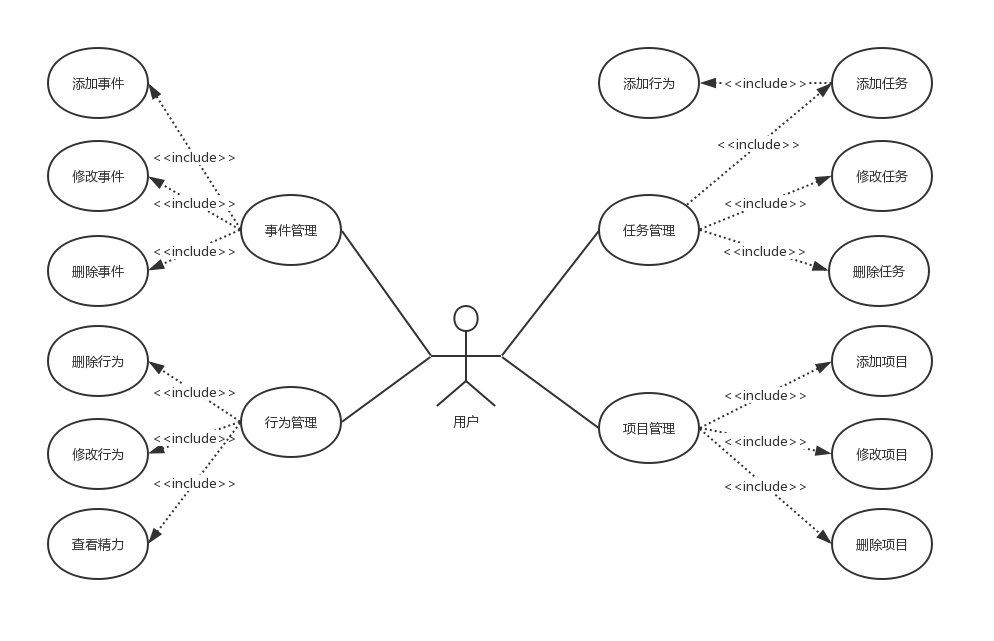
\includegraphics[width=\textwidth]{figure/uml/use_case.png}}
	\caption{任务计划及时间管理系统总用例图}
    \label{fig:use_case}
\end{figure}

图\ref{fig:use_case}基本包含了本系统的所有基本用例,
其中行为管理是根据需求分析得到的用于记录任务完成情况和精力分配的工具,
更为细致的用例描述见以下表格分析。

\begin{table}
	\centering
	\caption{用户添加任务用例描述表}
	\begin{tabular}{l|p{8cm}} \toprule
	  项目 & 内容说明 \\
	  \midrule
	  用例名称 & 用户添加任务 \\
	  参与者 & 用户 \\
	  前提条件 & 无 \\
	  前置操作 & 用户处于主界面状态 \\
	  后置操作 & 用户设置好任务信息后跳转回原界面 \\
	  合法流程 & 用户点击收件箱添加任务或长按收件箱添加任务,
	  设置好任务信息后点击保存 \\
	  异常情况举例 & 数据库或手机内部存储已满,无法添加 \\
	  \bottomrule
	\end{tabular}
\end{table}

\begin{table}
	\centering
	\caption{用户选择任务依赖关系用例描述表}
	\begin{tabular}{l|p{8cm}} \toprule
	  项目 & 内容说明 \\
	  \midrule
	  用例名称 & 用户选择任务依赖关系 \\
	  参与者 & 用户 \\
	  前提条件 & 用户已创建项目且项目中已含有任务 \\
	  前置操作 & 用户添加任务 \\
	  后置操作 & 跳转回添加任务界面 \\
	  合法流程 & 用户点击添加任务,选择合适的项目进行归类,
	  选择同一项目中的其他任务设置依赖关系 \\
	  异常情况举例 & 由于已经通过算法帮助用户排除了可能出现的
	  依赖关系形成环的情况,故在满足前提条件的情况下,基本无异常情况出现 \\
	  \bottomrule
	\end{tabular}
\end{table}

\begin{table}
	\centering
	\caption{用户完成任务用例描述表}
	\begin{tabular}{l|p{8cm}} \toprule
	  项目 & 内容说明 \\
	  \midrule
	  用例名称 & 用户选用户完成任务 \\
	  参与者 & 用户 \\
	  前提条件 & 用户已创建任务 \\
	  前置操作 & 用户添加任务 \\
	  后置操作 & 保持原界面或添加行为界面 \\
	  合法流程 & 用户点击完成任务,若任务未被分割,则直接完成,
	  若任务已被分割,则进入用户添加行为界面 \\
	  异常情况举例 & 数据库或手机内部存储已满,无法添加行为 \\
	  \bottomrule
	\end{tabular}
\end{table}

\begin{table}
	\centering
	\caption{用户添加事件用例描述表}
	\begin{tabular}{l|p{8cm}} \toprule
	  项目 & 内容说明 \\
	  \midrule
	  用例名称 & 用户添加事件 \\
	  参与者 & 用户 \\
	  前提条件 & 用户已授权系统日历使用权限 \\
	  前置操作 & 用户位于今日界面 \\
	  后置操作 & 保持原界面 \\
	  合法流程 & 用户未授权系统日历则弹出对话框授权使用,
	  若已授权则弹出添加事件的界面并进行设置 \\
	  异常情况举例 & 用户未授权系统日历,无法添加事件 \\
	  \bottomrule
	\end{tabular}
\end{table}

对于用户的需求进行分析后,发现任务这一实体的粒度不够细,需要再进行细化
也就是之前提到的行为,通过行为,我们可以更加细腻的了解用户在每个时间段的状态
便于以后的统计和分析,具体如图\ref{fig:activity}。

\begin{figure}
	\centering
	\makebox[\textwidth]{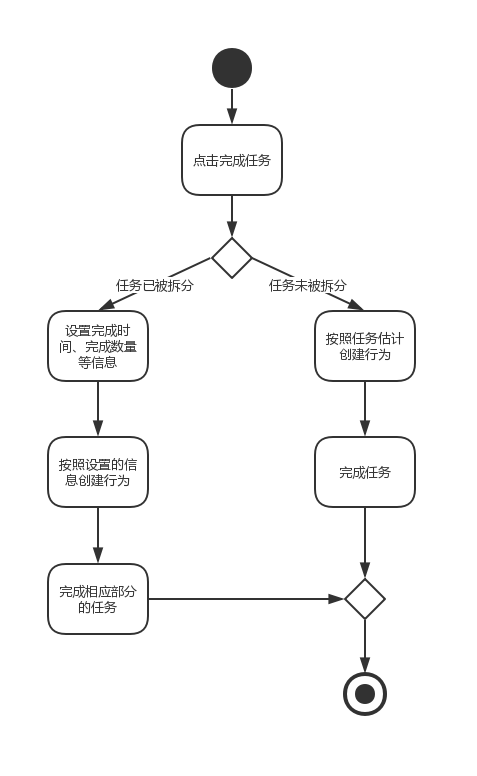
\includegraphics[height=12cm]{figure/uml/activity.png}}
	\caption{用户选择完成任务的活动图}
    \label{fig:activity}
\end{figure}

\section{其他需求}
\subsection{用户界面}
本系统的用户界面采用统一的GUI界面,并保持与iOS 系统应用风格的一致性,
其中出现的所有错误信息和提示信息均采用与系统风格统一的标准提示框。

\subsection{通讯接口}
\begin{itemize}
	\item 预留与Apple 服务器通讯并进行同步的iCloud 服务接口。
	\item 日常使用中可以不依赖网络使用,确保随时可用。
	\item 与其他日程管理类的软件通用接口:如系统日历,iCal通用日历信息文件。
	\item 与其他即时通讯类软件的交互接口:如文字信息入口等。
\end{itemize}

\subsection{性能需求}
\begin{itemize}
	\item 客户端一般响应时间不超过0.1秒。
	\item 任务统计时间不超过0.5秒。
\end{itemize}

\subsection{安全性需求}
\begin{itemize}
	\item 数据备份:允许用户进行数据的备份和恢复,以弥补数据的破坏和丢失。
	\item 加密:可以设置需要指纹或密码进入系统。
\end{itemize}

\subsection{可用性需求}
\begin{itemize}
	\item 控制必录入项:本系统能够对必须录入的内容进行控制,
	确保信息录入的完整。同时对必录入项进行有效的统一的提示,如使保存按钮不可用等。
	\item 容错能力:系统具有一定的容错和抗干扰能力,在非硬件故障或非通讯故障时,
	系统能够保证正常运行,并有足够的提示信息帮助用户有效正确地完成任务。
	\item 对于删除等具有破坏性的操作,提供撤销操作或予以提示。
\end{itemize}
%# -*- coding: utf-8-unix -*-
% !TEX program = xelatex
% !TEX root = ../thesis.tex
% !TEX encoding = UTF-8 Unicode
\chapter{系统设计}
完成系统的定义阶段之后,便进入了系统的设计阶段,
主要完成对系统的结构设计、系统模块设计与数据库表结构设计。
\section{系统框架结构设计}
本系统为满足不依赖网络、随时可用和安全性的特点,采用单用户体系结构,
本框架是我在iOS已有框架(Core Data和Event Kit)
的基础上融合而来,这两个框架都和Apple的服务紧密结合,方便今后对其进行扩展。
基本框架结构如图\ref{fig:level}所示。

\begin{figure}[!htbp]
	\centering
	\makebox[\textwidth]{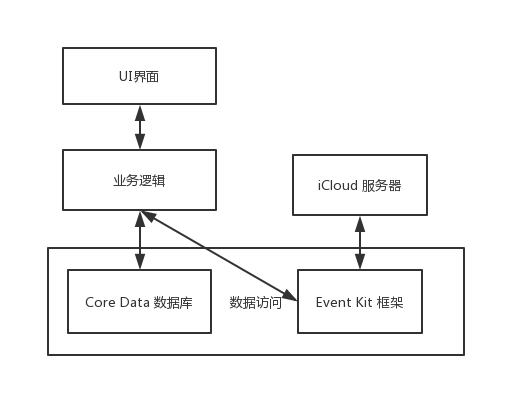
\includegraphics[height=8cm]{figure/level.png}}
	\caption{系统框架结构示意图}
    \label{fig:level}
\end{figure}

Core Data 是Apple提供的持久化数据的方案,一般来说,底层使用的是 Sqlite 数据库,如图\ref{fig:core_data}所示。
\begin{figure}[!htbp]
	\centering
	\makebox[\textwidth]{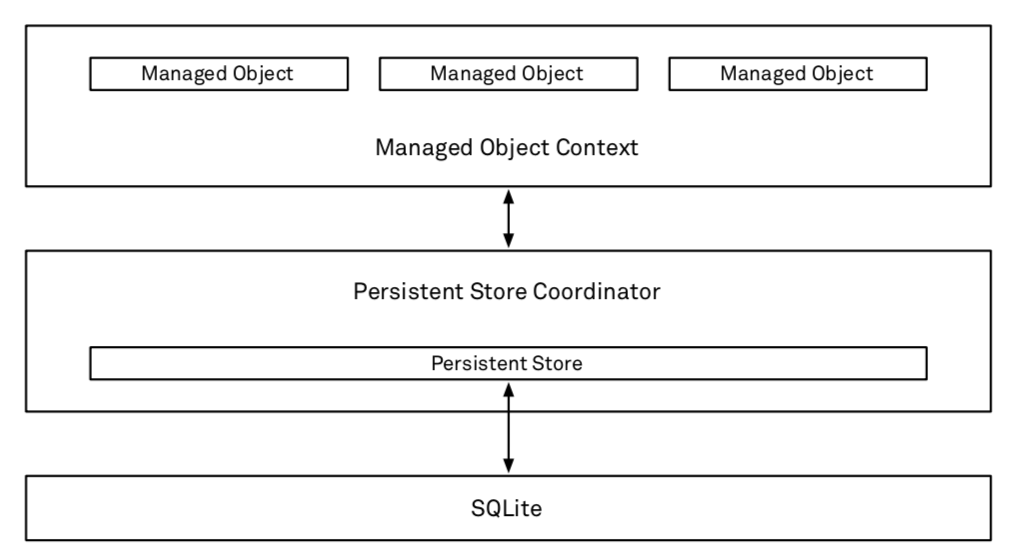
\includegraphics[height=6cm]{figure/core_data.png}}
	\caption{Core Data 结构示意图}
    \label{fig:core_data}
\end{figure}

\section{系统模块设计}
为保证系统的可拓展性和开发的便利,将系统分解为几个主要模块,如图\ref{fig:part}。
\begin{figure}[!htbp]
	\centering
	\makebox[\textwidth]{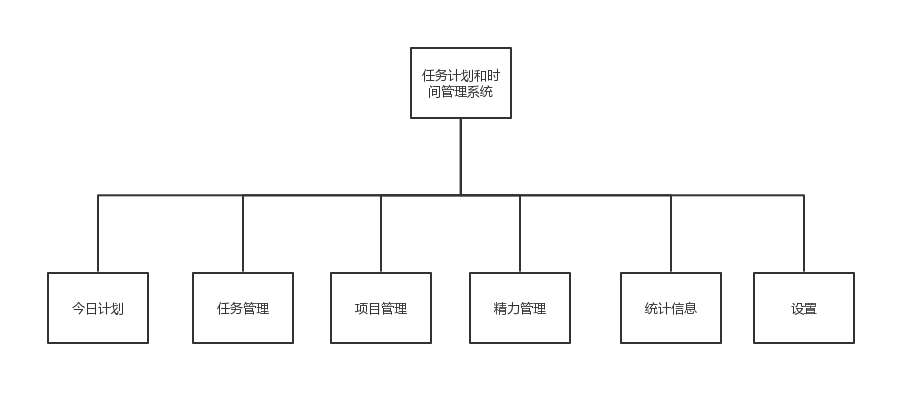
\includegraphics[width=\textwidth]{figure/part.png}}
	\caption{系统模块结构图}
    \label{fig:part}
\end{figure}

从图中可以看出任务计划及时间管理系统的架构设计,可以分为六个模块,
今日计划模块、任务管理模块、项目管理模块、精力管理模块、统计信息模块、设置模块,
系统通过用户输入获取信息,将信息保存到本地的数据库或系统的EventKit中,
再通过业务逻辑将信息经过排序、筛选等处理后进行展示。
其中每个模块均可直接通过主界面到达,将系统拆分为各个模块后,
降低了系统的耦合性,增强了系统的可拓展性。

\section{数据库设计}

\subsection{系统实体关系图}
由于Core Data会通过数据表之间的概念数据模型和他们之间的关系生成相应的物理模型(包括ID和主外建等),
无需开发者生成具体的物理模型。
图\ref{fig:e-r}中出现的事件和日历均为iOS系统自带的实体,也无需保存入Core Data 数据库中。
Core Data中的数据实体如图\ref{fig:core-data}所示。
\begin{figure}[!htbp]
	\centering
	\makebox[\textwidth]{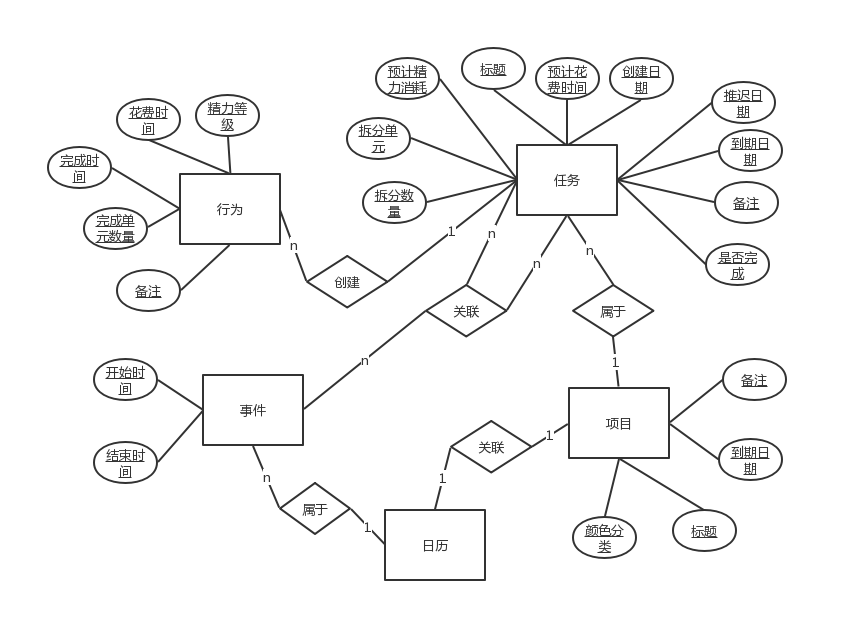
\includegraphics[width=\textwidth]{figure/e-r.png}}
	\caption{实体关系图}
    \label{fig:e-r}
\end{figure}

\begin{figure}[!htbp]
	\centering
	\makebox[\textwidth]{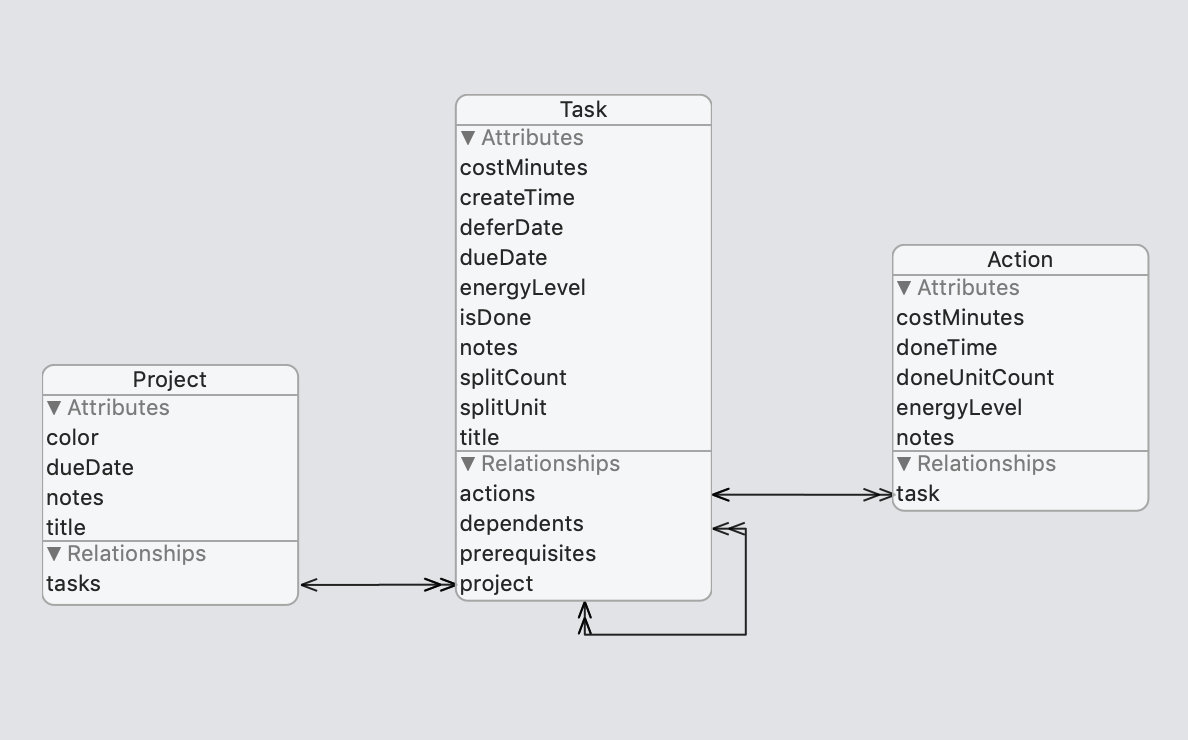
\includegraphics[width=\textwidth]{figure/relationship.png}}
	\caption{Core Data 数据实体及关系图}
	\label{fig:core-data}
\end{figure}

\subsection{系统数据表}

\begin{table}[H]
  \centering
  \caption{任务表}
  \begin{tabular}{ccccccc} \toprule
	序号 & 列名 & 数据类型 & 允许空 & 说明 & 备注 \\
	\midrule
	1 & costMinutes & Integer32 & 否 & 花费时间 & 无 \\
	2 & createTime & Date & 否 & 创建时间 & 无 \\
	3 & deferDate & Date & 否 & 推迟日期 & 无 \\
	4 & dueDate & Date & 否 & 到期时间 & 无 \\
	5 & energyLevel & Integer16 & 否 & 精力等级 & 无 \\
	6 & isDone & Boolean & 否 & 是否完成 & 无 \\
	7 & notes & String & 否 & 备注 & 无 \\
	8 & splitCount & Integer32 & 否 & 拆分数量 & 无 \\
	9 & splitUnit & String & 否 & 拆分单位 & 无 \\
	10 & title & String & 否 & 标题 & 无 \\
	\bottomrule
  \end{tabular}
\end{table}

\begin{table}[H]
	\centering
	\caption{项目表}
	\begin{tabular}{ccccccc} \toprule
	  序号 & 列名 & 数据类型 & 允许空 & 说明 & 备注 \\
	  \midrule
	  1 & color & Transformable & 否 & 花费时间 & UIColor \\
	  2 & dueDate & Date & 否 & 到期时间 & 无 \\
	  3 & notes & String & 否 & 备注 & 无 \\
	  4 & title & String & 否 & 题目 & 无 \\
	  \bottomrule
	\end{tabular}
\end{table}

\begin{table}[H]
	\centering
	\caption{行为表}
	\begin{tabular}{ccccccc} \toprule
	  序号 & 列名 & 数据类型 & 允许空 & 说明 & 备注 \\
	  \midrule
	  1 & costMinutes & Integer32 & 否 & 花费时间 & UIColor \\
	  2 & doneTime & Date & 否 & 完成时间 & 无 \\
	  3 & doneUnitCount & Integer32 & 否 & 完成数量 & 无 \\
	  4 & energyLevel & Integer16 & 否 & 精力花费 & 无 \\
	  5 & notes & String & 否 & 备注 & 无 \\
	  \bottomrule
	\end{tabular}
\end{table}



\backmatter % 文后无编号部分

\makeatletter

% 致谢
%# -*- coding: utf-8-unix -*-
% !TEX program = xelatex
% !TEX root = ../thesis.tex
% !TEX encoding = UTF-8 Unicode
%TC:ignore
\begin{thanks}

大学四年的学习生活即将结束,在本次毕业设计完成之际,
我要特别感谢我的指导老师李丽萍老师,老师秉承认真负责的工作态度,
在整个毕业设计过程中定时督促、检查我的系统完成情况,
从中指出我的不足之处,在我遇到困难时给予耐心的指导。
我能够完成系统的设计、编码和论文,还要感谢同学们的无私帮助。
非常感谢他们能够抽出时间,帮助我发现问题,解决问题,给出了很多有用的建议和补充。
最后,我由衷的感谢所有教导过我的老师们,
你们严谨的治学风格,让我很好的学习了专业知识;
你们独特的人格魅力,感染教导我为人处事。
还要感谢我的母校——上海第二工业大学四年来对我的精心培养,
让我能够变的更加出色,让我有自信成为社会的有用之才。

\end{thanks}
%TC:endignore
 

% 参考资料
\printbibliography[heading=bibintoc]

\makeatother

\end{document}
